\documentclass[12pt,a4paper,UTF8]{article}

\usepackage[titletoc]{appendix}
\usepackage{xeCJK}
\usepackage{amsmath}
\usepackage{array}
\usepackage{bm}
\usepackage{booktabs}
\usepackage{caption}
\usepackage{cite}
\usepackage{comment}
\usepackage{float}
\usepackage{fontspec} % xelatex限定
\usepackage{geometry}
\usepackage{graphicx}
\usepackage{indentfirst}
% \usepackage[utf8]{inputenc} % 非xelatex编译,显式指定文件编码为utf8
\usepackage{listings}
\usepackage{longtable}
\usepackage{mathtools}
\usepackage{multicol}
\usepackage{multirow}
\usepackage{supertabular}
\usepackage{subcaption}
\usepackage{tabu}
\usepackage{ulem}
\usepackage{url}
\usepackage{xcolor}
\usepackage{nccmath} % だが align* は nccmath が無くても使えるので敢えて両方書いた。
% \usepackage{CJKutf8}
% \usepackage{hyperref}

\geometry{a4paper,left=2.5cm,right=2.5cm,top=2.5cm,bottom=2.5cm}
\defaultCJKfontfeatures{Scale=1.2}
\linespread{1.5}

%% Define a new 'leo' style for the package that will use a smaller font.
\makeatletter
\def\url@leostyle{%
  \@ifundefined{selectfont}{\def\UrlFont{\sf}}{\def\UrlFont{\small\ttfamily}}}
\makeatother
\urlstyle{leo} % Now actually use the newly defined style.


\renewcommand{\contentsname}{\centering{目录}}
\renewcommand{\abstractname}{\large{摘要}}
\def\tablename{表}
\def\figurename{图}
\renewcommand{\thetable}{\thesection.\arabic{table}}
\renewcommand{\thefigure}{\thesection.\arabic{figure}}
\renewcommand{\multirowsetup}{\centering}
\renewcommand{\appendixname}{附录~\Alpha{section}}
\renewcommand{\refname}{参考文献}

\everymath{\displaystyle}
\bibliographystyle{plain}


\lstdefinestyle{BASH}{
    breaklines=true,                                     % 自动换行
    columns=fixed,
    extendedchars=true,                                  % lets you use non-ASCII characters; for 8-bits encodings only, does not work with UTF-8
    frame=shadowbox,                                     % 设置背景边框
    numbers=left,                                        % 在左侧显示行号
    numberstyle=\footnotesize\color{darkgray},           % 设定行号格式
    showstringspaces=false,                              % 不显示字符串中的空格
    tabsize=4,	                                         % 设置tab长度
}
\lstdefinestyle{tinyBASH}{
    breaklines=true,                                     % 自动换行
    basicstyle=\footnotesize\ttfamily,
    columns=fixed,
    extendedchars=true,                                  % lets you use non-ASCII characters; for 8-bits encodings only, does not work with UTF-8
    frame=shadowbox,                                     % 设置背景边框
    numbers=left,                                        % 在左侧显示行号
    numberstyle=\footnotesize\color{darkgray},           % 设定行号格式
    showstringspaces=false,                              % 不显示字符串中的空格
    tabsize=4,	                                         % 设置tab长度
}
\lstdefinestyle{Python}{
    breaklines=true,                                     % 自动换行
    captionpos=b,                                        % sets the caption-position to bottom
    columns=fixed,
    commentstyle=\it\color[RGB]{0,96,96},                % 设置代码注释的格式
    % extendedchars=true,                                  % lets you use non-ASCII characters; for 8-bits encodings only, does not work with UTF-8
    frame=shadowbox,                                     % 设置背景边框
    keywordstyle=\bfseries\color[RGB]{40,40,255},        % 设定关键字颜色
    language=Python,                                     % 设置语言
    numbers=left,                                        % 在左侧显示行号
    numberstyle=\footnotesize\color{darkgray},           % 设定行号格式
    stringstyle=\rmfamily\slshape\color[RGB]{128,0,0},   % 设置字符串格式
    tabsize=4,	                                         % 设置tab长度
}

\lstdefinestyle{CPP}{
    %backgroundcolor=\color[RGB]{245,245,244},           % 设定背景颜色
    breaklines=true,                                     % 自动换行
    captionpos=b,                                        % sets the caption-position to bottom
    columns=fixed,
    commentstyle=\it\color[RGB]{0,96,96},                % 设置代码注释的格式
    extendedchars=true,                                  % lets you use non-ASCII characters; for 8-bits encodings only, does not work with UTF-8
    frame=shadowbox,                                     % 设置背景边框
    keywordstyle=\bfseries\color[RGB]{40,40,255},        % 设定关键字颜色
    language=c++,                                        % 设置语言
    numbers=left,                                        % 在左侧显示行号
    numberstyle=\footnotesize\color{darkgray},           % 设定行号格式
    showstringspaces=false,                              % 不显示字符串中的空格
    stringstyle=\rmfamily\slshape\color[RGB]{128,0,0},   % 设置字符串格式
    tabsize=4,	                                         % 设置tab长度
    title=\lstname,                                      % show the filename of files included with \lstinputlisting; also try caption instead of title
    morekeywords={alignas,continute,friend,register,true,alignof,decltype,goto,
        reinterpret_cast,try,asm,defult,if,return,typedef,auto,delete,inline,short,
        typeid,bool,do,int,signed,typename,break,double,long,sizeof,union,case,
        dynamic_cast,mutable,static,unsigned,catch,else,namespace,static_assert,using,
        char,enum,new,static_cast,virtual,char16_t,char32_t,explict,noexcept,struct,
        void,export,nullptr,switch,volatile,class,extern,operator,template,wchar_t,
        const,false,private,this,while,constexpr,float,protected,thread_local,
        const_cast,for,public,throw,std},
    emph={map,set,multimap,multiset,unordered_map,unordered_set,
        unordered_multiset,unordered_multimap,vector,string,list,deque,
        array,stack,forwared_list,iostream,memory,shared_ptr,unique_ptr,
        random,bitset,ostream,istream,cout,cin,endl,move,default_random_engine,
        uniform_int_distribution,iterator,algorithm,functional,bing,numeric},
}

\lstdefinestyle{QT}{
    %backgroundcolor=\color[RGB]{245,245,244},           % 设定背景颜色
    breaklines=true,                                     % 自动换行
    captionpos=b,                                        % sets the caption-position to bottom
    columns=fixed,
    commentstyle=\it\color[RGB]{0,96,96},                % 设置代码注释的格式
    extendedchars=true,                                  % lets you use non-ASCII characters; for 8-bits encodings only, does not work with UTF-8
    frame=shadowbox,                                     % 设置背景边框
    keywordstyle=\bfseries\color[RGB]{40,40,255},        % 设定关键字颜色
    language=c++,                                        % 设置语言
    numbers=left,                                        % 在左侧显示行号
    numberstyle=\footnotesize\color{darkgray},           % 设定行号格式
    stringstyle=\rmfamily\slshape\color[RGB]{128,0,0},   % 设置字符串格式
    showstringspaces=false,                              % 不显示字符串中的空格
    tabsize=4,	                                         % 设置tab长度
    title=\lstname,                                      % show the filename of files included with \lstinputlisting; also try caption instead of title
    morekeywords={alignas,continute,friend,register,true,alignof,decltype,goto,
        reinterpret_cast,try,asm,defult,if,return,typedef,auto,delete,inline,short,
        typeid,bool,do,int,signed,typename,break,double,long,sizeof,union,case,
        dynamic_cast,mutable,static,unsigned,catch,else,namespace,static_assert,using,
        char,enum,new,static_cast,virtual,char16_t,char32_t,explict,noexcept,struct,
        void,export,nullptr,switch,volatile,class,extern,operator,template,wchar_t,
        const,false,private,this,while,constexpr,float,protected,thread_local,
        const_cast,for,public,throw,std,bind,function,
        Q_OBJECT,QDialog,QUdpSocket,QTcpSocket,QHostAddress,QNetworkDatagram,QTcpServer,
        QByteArray,QString,QStringList,QList,QSet,QMap,
        quint,qint64,uintptr_t,
        connect,signals,slots,SIGNAL,SLOT},
    emph={map,set,multimap,multiset,unordered_map,unordered_set,
        unordered_multiset,unordered_multimap,vector,string,list,deque,
        array,stack,forwared_list,iostream,memory,shared_ptr,unique_ptr,
        random,bitset,ostream,istream,cout,cin,endl,move,default_random_engine,
        uniform_int_distribution,iterator,algorithm,functional,bing,numeric},
}

\lstdefinestyle{MASM}{
    breaklines=true,                                     % 自动换行
    captionpos=b,                                        % sets the caption-position to bottom
    columns=fixed,
    commentstyle=\it\color[RGB]{0,96,96},                % 设置代码注释的格式
    extendedchars=true,                                  % lets you use non-ASCII characters; for 8-bits encodings only, does not work with UTF-8    
    frame=shadowbox,                                     % 设置背景边框
    keywordstyle=\bfseries\color[RGB]{40,40,255},        % 设定关键字颜色
    language=[x86masm]Assembler,                         % 设置语言
    numbers=left,                                        % 在左侧显示行号
    numberstyle=\footnotesize\color{darkgray},           % 设定行号格式
    stringstyle=\rmfamily\slshape\color[RGB]{128,0,0},   % 设置字符串格式
    showstringspaces=false,                              % 不显示字符串中的空格
    tabsize=4,	                                         % 设置tab长度
    title=\lstname,                                      % show the filename of files included with \lstinputlisting; also try caption instead of title
    morekeywords={CDQE,CQO,CMPSQ,CMPXCHG16B,JRCXZ,LODSQ,MOVSXD, % 
        POPFQ,PUSHFQ,SCASQ,STOSQ,IRETQ,RDTSCP,SWAPGS, % 
        .code,.def,.file,.type,.ended,.scl,.section,.ascii,.text,.globl,.ident,.rodata,
        .sch_proc,.sch_pushreg,.sch_setframe,.sch_stackalloc,.sch_endprologue,.sch_endproc,
        pushq,popq,movq,movl,addq,subq,leaq,invoke,start,addr,
        rax,rdx,rcx,rbx,rsi,rdi,rip,rsp,rbp, % 
        r8,r8d,r8w,r8b,r9,r9d,r9w,r9b, % 
        r10,r10d,r10w,r10b,r11,r11d,r11w,r11b, % 
        r12,r12d,r12w,r12b,r13,r13d,r13w,r13b, % 
        r14,r14d,r14w,r14b,r15,r15d,r15w,r15b}
}
\newcommand{\includecode}[2][c]{\lstinputlisting[caption=#2, escapechar=, style=#1]{#2}}



% \setcounter{table}{0}
% \setcounter{figure}{0}

% \lstinputlisting[style=CPP]{src/main.cpp}

% \begin{figure}[H]
%     \centering
%     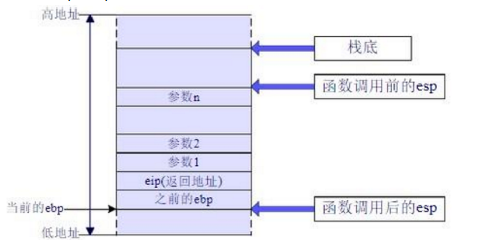
\includegraphics[width = .75\linewidth]{img/1.png}
%     \caption{预处理结果(部分)}
%     \label{fig::figure2}
% \end{figure}


% 结果如表\ref{tab::table2}:
% \begin{table}[htbp]
%     \begin{center}
%         \begin{tabular}{c c c}
%             \toprule
%             优化等级 & 二进制文件大小(Byte) &  执行时间(s)\\
%             \midrule
%             不优化 & 13992 & 36.090 \\
%             O1 & 13344 & 10.562\\
%             O2 & 13344 & 9.925\\
%             Os & 13344 & 8.899\\
%             O3 & 13344 & 8.350\\
%             Ofast & 14800 & 8.094\\
%             \bottomrule
%         \end{tabular}
%         \caption{各等级优化测试结果}\label{tab::table2}
%     \end{center}
% \end{table}

% \begin{equation}
%     \begin{split}
%         id     & \rightarrow char\ |\ id\ digit\ |\ id\ char \\
%         digit  & \rightarrow 0\ |\ 1\ |\ 2\ |\ 3\ |\ 4\ |\ 5\ |\ 6\ |\ 7\ |\ 8\ |\ 9 \\
%         char   & \rightarrow \_\ |\ letter \\
%         letter & \rightarrow A\ |\ B\ |\ ...\ |\ Z\ |\ a\ |\ b\ |\ ...\ |\ z \\
%     \end{split}
% \end{equation}


\begin{document}

\title{Lab 1: Booting a PC——Part1\&2}
\author{罗宸、朱勋建、朱志成、赵审铎、罗思唯、吴昆默}
\date{\today}

\maketitle

\begin{abstract}
    \setlength{\parindent}{2em}
    本次实验取自MIT\ 6.828\ Lab1的前两个部分。第一部分主要熟悉x86汇编语言、QEMU的x86 模拟器和PC开机的引导过程。
    第二部分主要检查内核的引导加载程序。

    \textbf{关键词:qemu、boot loader、JOS kernel}
\end{abstract}


% \section{引言}


\section{实验环境与工具}

本实验使用Ubuntu\ 18.04系统与qemu\ 6.828进行。


\section{练习一\ GNU assembler}

MASM汇编微软定义的汇编语言。AT\&T汇编是GNU的开发者定义的汇编语言。
GNU汇编程序是GNU操作系统的默认汇编程序。它处理多个架构并支持多种汇编语言语法。
主要用于汇编GNU c编译器的输出以供链接器使用,因此它可以被视为tigcc包的内部部分。
然而,它可能被称为一个独立的程序,GNU汇编试图使as-assemble能够正确地组装同一台机器的其他汇编程序。
任何异常都有明确的记录。GNU assambler可执行文件称为as,是UNIX汇编程序的基本名称。


\section{问题一\ Boot Loader}

    \subsection{}
	处理器什么时候开始执行 32 位代码?如何完成的从 16 位到 32 位模式的切换?

	阅读boot.asm中的代码与注释,".code16"段为实模式,".code32"段为保护模式,
	由此可知,处理器在命令ljmp\ \$PROT\_MODE\_CSEG, \$protcseg之后开始执行32位代码。

	这一切换过程是通过如下命令实现的
	\begin{lstlisting}[style=MASM]
  # Switch from real to protected mode, using a bootstrap GDT
  # and segment translation that makes virtual addresses 
  # identical to their physical addresses, so that the 
  # effective memory map does not change during the switch.
  lgdt    gdtdesc
    7c1e:	0f 01 16             	lgdtl  (%esi)
    7c21:	64 7c 0f             	fs jl  7c33 <protcseg+0x1>
  movl    %cr0, %eax
    7c24:	20 c0                	and    %al,%al
  orl     $CR0_PE_ON, %eax
    7c26:	66 83 c8 01          	or     $0x1,%ax
  movl    %eax, %cr0
    7c2a:	0f 22 c0             	mov    %eax,%cr0
	\end{lstlisting}

	其中加载了全局描述符表,然后将cr0中的PE位置1,从而实现从实模式到保护模式的转换。

    \subsection{}
	引导加载程序 boot loader 执行的最后一个指令是什么,加载的内核的第一个指令是什么?

	boot loader执行的最后一条指令为$call\ \ *0x10018$,调用了ELF的头部,实现跳转到kernel。

	内核执行的第一条指令从kernel.asm中找,如下
	\begin{lstlisting}[style=MASM]
.globl entry
entry:
   movw	$0x1234,0x472			# warm boot
	\end{lstlisting}
    \subsection{}
	内核执行的第一条指令在哪?

	调用objdump\ -f\ obj/kern/kernel,得到
	\begin{lstlisting}[style=BASH]
$ objdump -f obj/kern/kernel

obj/kern/kernel:     file format elf32-i386
architecture: i386, flags 0x00000112:
EXEC_P, HAS_SYMS, D_PAGED
start address 0x0010000c
.........
	\end{lstlisting}

	由此可知内核的第一条指令的地址为0x0010000c。

	\subsection{}
	boot loader如何决定为了从磁盘获取整个内核必须读取多少扇区?在哪里可以找到这些信息?

	boot loader会从硬盘中读入ELF File Header,对应代码在boot/main.c的bootmain函数中:
	\begin{lstlisting}[style=CPP]
// read 1st page off disk
readseg((uint32_t) ELFHDR, SECTSIZE*8, 0);

// is this a valid ELF?
if (ELFHDR->e_magic != ELF_MAGIC)
	goto bad;

// load each program segment (ignores ph flags)
ph = (struct Proghdr *) ((uint8_t *) ELFHDR + ELFHDR->e_phoff);
eph = ph + ELFHDR->e_phnum;
for (; ph < eph; ph++)
	// p_pa is the load address of this segment (as well
	// as the physical address)
	readseg(ph->p_pa, ph->p_memsz, ph->p_offset);

// call the entry point from the ELF header
// note: does not return!
((void (*)(void)) (ELFHDR->e_entry))();
	\end{lstlisting}

	从硬盘中读取ELFHDR,通过设定好的魔法数字来检验ELF头的有效性。

	可以看到,由ELFHDR的地址+程序头表的文件偏移e\_phoff能得到开始其中保存的起始程序头的地址ph,
	eph = ph + ELF Header中总的程序头个数e\_phnum为结束地址。

	利用ph和eph可遍历每一个程序头,并依次从中读取出kernel的内容。


\section{问题二\ Kernel}

	\subsection{}
	printf.c对console.c的接口是cprintf(const char *fmt),在console.c中需要输出一个字符串时直接把字符串作参数(可以以print格式添加变量)调用即可,
	返回输出字符串的长度。但事实上printf.c中仅仅提供一个封装的接口,在cprintf(const char *fmt)被调用后,
	会调用定义在printfmt.c中的vprintfmt(void (*putch)(int, void*),void *putdat, const char *fmt, va\_list ap)进行逐字分析,以决定是处理控制符还是输出常量部分。

	最后打印工作交由定义在console.c中的cputchar(int c)处理,cputchar(int c)会调用serial\_init(void),lpt\_putc(int c),cga\_init(void)三个函数来完成具体的打印工作。

	\subsection{}
	\begin{lstlisting}[style=CPP]
if (crt_pos >= CRT_SIZE) {
	int i;
	memmove(crt_buf, crt_buf + CRT_COLS, (CRT_SIZE - CRT_COLS) * sizeof(uint16_t));
	for (i = CRT_SIZE - CRT_COLS; i < CRT_SIZE; i++)
		crt_buf[i] = 0x0700 | ' ';
	crt_pos -= CRT_COLS;
}
	\end{lstlisting}

	这段代码的目的是缓冲区满时清除一部分留出空间,可以理解成一页写满时自动下拉一行。
	比如设一页有25行,每行可放80个字符,则CRT\_SIZE=25*80=2000,CRT\_CLOS=80。
	当检测到crt\_pos$>$CRT\_SIZE,即光标位置超出屏幕外时,将缓冲区(crt\_buf)中后24行复制到前24行,最后一行以'\ '填充。
	最后将光标位置上移一行。

\section{作业一\ printf()}

补全输出"\%o"格式字符串的代码。

首先分析kern/printf.c,lib/printfmt.c和kern/console.c三者的关系。
由代码上方的注释可知kern/printf.c中的vcprintf,cprintf函数都调用了lib/printfmt.c中的vprintfmt函数:

\begin{lstlisting}[style=CPP]
int
vcprintf(const char *fmt, va_list ap)
{
	int cnt = 0;
	vprintfmt((void*)putch, &cnt, fmt, ap);
	return cnt;
}    
\end{lstlisting}

经查阅资料后可知它的四个输入参数中(void*)putch(int,\ void*)为函数指针,一般调用输出到屏幕上的函数。
void\ *putdat是输入字符要放的内存地址指针。const\ char\ *fmt 是格式化字符串。va\_list\ ap为多个输入参数。

kern/printf.c中的putch函数调用kern/console.c的cputchar函数。lib/printfmt.c中也有putch函数。所以 kern/printf.c 和 lib/printfmt.c 依赖于kern/console.c。

之后去分析kern/console.c。

kern/console.c中的cputchar函数调用了cons\_putc函数:

\begin{lstlisting}[style=CPP]
// output a character to the console
static void
cons_putc(int c)
{
	serial_putc(c);
	lpt_putc(c);
	cga_putc(c);
}
\end{lstlisting}

cons\_putc的功能是输出一个字符到控制台。由serial\_putc,lpt\_putc和cga\_putc这三个函数组成。

先分析serial\_putc函数:

\begin{lstlisting}[style=CPP]
static void
serial_putc(int c)
{
	int i;
	for (i = 0;
	     !(inb(COM1 + COM_LSR) & COM_LSR_TXRDY) && i < 12800;
	     i++)
		delay();
	outb(COM1 + COM_TX, c);
}
\end{lstlisting}

它控制的是端口0x3F8,inb内联汇编函数读取的是 COM1 + COM\_LSR = 0x3FD 端口,
outb内联汇编函数输出到了COM1 + COM\_TX = 0x3F8端口。在 inb(COM1 + COM\_LSR) 之后,
有 \& COM\_LSR\_TXRDY 这个操作。!(inb(COM1 + COM\_LSR) \& COM\_LSR\_TXRDY)是为了查看读入的数据的第6位,
也就 PORTS.LST中03FD中提到的bit 5是否为1。如果为1,上面的语句结果就是0,停止for循环。
这个bit 5是判断发送数据缓冲寄存器是否为空。outb 是将端口 0x3F8 的内容输出到 c。
当0x3F8被写入数据,它作为发送数据缓冲寄存器,数据是要发给串口。所以serial\_putc是为了把一个字符输出到串口。

再分析lpt\_putc函数:

\begin{lstlisting}[style=CPP]
static void
lpt_putc(int c)
{
	int i;
	for (i = 0; !(inb(0x378+1) & 0x80) && i < 12800; i++)
		delay();
	outb(0x378+0, c);
	outb(0x378+2, 0x08|0x04|0x01);
	outb(0x378+2, 0x08);
}
\end{lstlisting}

它的作用是将字符给并口设备。

最后分析cga\_putc函数:

\begin{lstlisting}[style=CPP]
static void
cga_putc(int c)
{
	// if no attribute given, then use black on white
	if (!(c & ~0xFF))
		c |= 0x0700;
	switch (c & 0xff) {
	case '\b':
		if (crt_pos > 0) {
			crt_pos--;
			crt_buf[crt_pos] = (c & ~0xff) | ' ';
		}
		break;
	case '\n':
		crt_pos += CRT_COLS;
		/* fallthru */
	case '\r':
		crt_pos -= (crt_pos % CRT_COLS);
		break;
	case '\t':
		cons_putc(' ');
		cons_putc(' ');
		cons_putc(' ');
		cons_putc(' ');
		cons_putc(' ');
		break;
	default:
		crt_buf[crt_pos++] = c;		/* write the character */
		break;
	}
	// What is the purpose of this?
	if (crt_pos >= CRT_SIZE) {
		int i;

		memmove(crt_buf, crt_buf + CRT_COLS, (CRT_SIZE - CRT_COLS) * sizeof(uint16_t));
		for (i = CRT_SIZE - CRT_COLS; i < CRT_SIZE; i++)
			crt_buf[i] = 0x0700 | ' ';
		crt_pos -= CRT_COLS;
	}
	/* move that little blinky thing */
	outb(addr_6845, 14);
	outb(addr_6845 + 1, crt_pos >> 8);
	outb(addr_6845, 15);
	outb(addr_6845 + 1, crt_pos);
}
\end{lstlisting}

其中!(c \& $\sim$ 0xFF) 用来检测是否在 0 255 之间。$\backslash$ b是退格键,让缓冲区 crt\_buf 的下标 crt\_pos 减1。
其他的同理,case都是格式操作。default是往缓冲区里写入字符c。当缓存超过CRT\_SIZE,就用memmove复制内存内容。
最后四句代码是将缓冲区的内容输出到显示屏。

最后是去实现"\%o"的格式化输出,在lib/printfmt.c中可以看到要填写的地方:

\begin{lstlisting}[style=CPP]
    // (unsigned) octal
    case 'o':
        // Replace this with your code.
        putch('X', putdat);
        putch('X', putdat);
        putch('X', putdat);
        break;
\end{lstlisting}

参考上面 case 'u' 中的写法,可以得出:
\begin{lstlisting}[style=CPP]
    case 'o':
        num = getuint(&ap, lflag);
        base = 8;
        goto number;
\end{lstlisting}

修改完以后保存,make\ clean之后运行,会发现启动以后,qemu里JOS启动时会出现:

\begin{figure}[H]
    \centering
    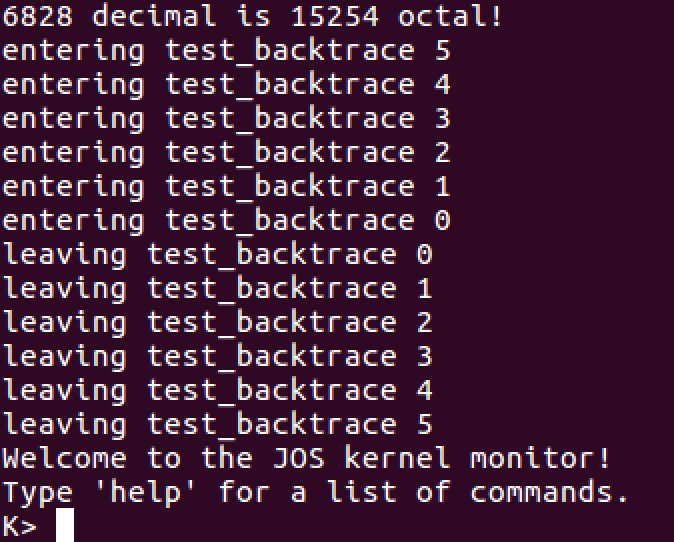
\includegraphics[width = .75\linewidth]{img/h1_1.png}
    \caption{printf("\%o")}
    \label{fig::figure1}
\end{figure}

可见第一行完成了十进制数6828转八进制。

\section{作业二}

\setcounter{table}{0}
\setcounter{figure}{0}

问题二要求实现mon\_backtrace()函数,显示ebp,eip和arg信息。

	\subsection{涉及属性}
	eip(返回指令指针):存储当前执行指令的下一条指令在内存中的偏移地址。

	ebp(基址指针):存储指向当前函数需要使用的参数的指针。

	esp (栈指针):存储指向栈顶的指针。

	在程序中,如果需要调用一个函数,首先会将函数需要的参数进栈,然后将 eip 中的内容进栈,
	也就是下一条指令在内存中的位置,这样在函数调用结束后便可以通过堆栈中的 eip 值。
	返回调用函数的程序,如下图所示
	\begin{figure}[H]
		\centering
		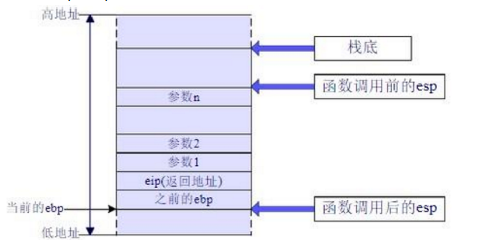
\includegraphics[width = .8\linewidth]{img/1.png}
		\caption{栈}
		\label{fig::figure2-1}
	\end{figure}

	\subsection{涉及函数}
	mon\_backtrace函数的原型在kern/monitor.c中
	\begin{lstlisting}[style=CPP]
int
mon_backtrace(int argc, char **argv, struct Trapframe *tf)
{
	return 0;
}
	\end{lstlisting}

	调用mon\_backtrace的函数test\_backtrace在kern/init.c中
	\begin{lstlisting}[style=CPP]
// Test the stack backtrace function (lab 1 only)
void
test_backtrace(int x)
{
	cprintf("entering test_backtrace %d\n", x);
	if (x > 0)
		test_backtrace(x-1);
	else
		mon_backtrace(0, 0, 0);
	cprintf("leaving test_backtrace %d\n", x);
}
	\end{lstlisting}

	kern/entry.s中提供的停止信息如下
	\begin{lstlisting}[style=CPP]
relocated:
# Clear the frame pointer register (EBP)
# so that once we get into debugging C code,
# stack backtraces will be terminated properly.
movl	$0x0,%ebp		# nuke frame pointer
	\end{lstlisting}

	即,进入内核监控后,stack\ tracers会被中止,mon\_backtrace和test\_backtrace的作用域失效,
	可确定当ebp值为0时停止题目要求信息的打印。

	read\_edp在inc/x86.h中
	\begin{lstlisting}[style=CPP]
static __inline uint32_t
read_ebp(void)
{
	uint32_t ebp;
	__asm __volatile("movl %%ebp,%0" : "=r" (ebp));
	return ebp;
}
	\end{lstlisting}

	则read\_edp的返回值类型为uint32\_t,对应可确定edp变量类型。

	\subsection{代码编写及执行情况}
	由上述描述,用格式符"\%08x"进行8位16进制的格式控制,编写代码如下:
	\begin{lstlisting}[style=CPP]
int
mon_backtrace(int argc, char **argv, struct Trapframe *tf)
{
	int i;
	cprintf("Stack backtrace:\n");
	uint32_t ebp = read_ebp();
	while ((int)ebp != 0)
	{
		cprintf("  ebp:0x%08x eip:0x%08x args:%08x %08x %08x %08x %08x", ebp,
		*((uint32_t *)ebp+1),*((uint32_t *)ebp+2),*((uint32_t *)ebp+3),
		*((uint32_t *)ebp+4),*((uint32_t *)ebp+5),*((uint32_t *)ebp+6));
	cprintf("\n");
	ebp = ((uint32_t *)ebp)[0];
	}
	return 0;
}
	\end{lstlisting}

	程序执行情况如下:
	\begin{figure}[H]
		\centering
		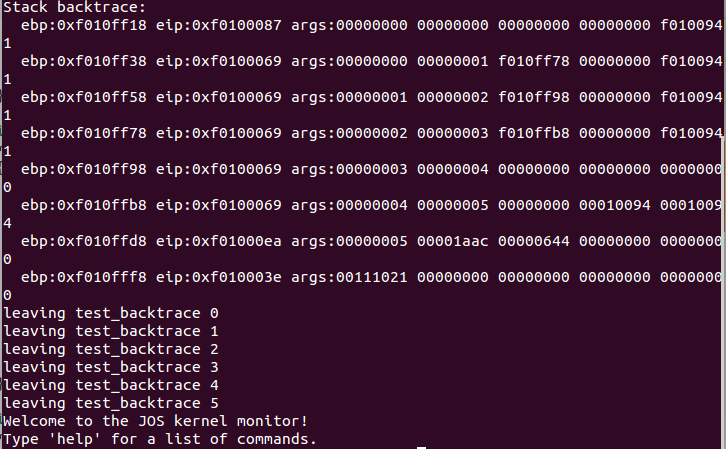
\includegraphics[width = .8\linewidth]{img/7.png}
		\caption{作业二结果}
		\label{fig::figure2-7}
	\end{figure}


\section{挑战作业}

\setcounter{table}{0}
\setcounter{figure}{0}

为每个eip显示源文件名函数名和行号。

为了输出eip的调试信息,根据题中信息,首先去kern/kdebug.h中查看定义:

\begin{lstlisting}[style=CPP]
// Debug information about a particular instruction pointer
struct Eipdebuginfo {
	const char *eip_file;	// Source code filename for EIP
	int eip_line;			// Source code linenumber for EIP
	const char *eip_fn_name;// Name of function containing EIP
							// -Note: not null terminated!
	int eip_fn_namelen;		// Length of function name
	uintptr_t eip_fn_addr;	// Address of start of function
	int eip_fn_narg;		// Number of function arguments
};

int debuginfo_eip(uintptr_t addr, struct Eipdebuginfo *info);	
\end{lstlisting}

然后根据注释查看inc/stab.h中stab的定义:
\begin{lstlisting}[style=CPP]
// Entries in the STABS table are formatted as follows.
struct Stab {
	uint32_t n_strx;	// index into string table of name
	uint8_t n_type;     // type of symbol
	uint8_t n_other;    // misc info (usually empty)
	uint16_t n_desc;    // description field
	uintptr_t n_value;	// value of symbol
};
\end{lstlisting}

根据函数debuginfo\_eip注释中的提示,添加函数stab\_binsearch的调用以搜索行号并完成设定:

\begin{lstlisting}[style=CPP]
stab_binsearch(stabs, &lline, &rline, N_SLINE, addr);
if(lline <= rline) {
	info->eip_line = stabs[rline].n_desc;
} else {
	info->eip_line = -1;
}
\end{lstlisting}

进一步修改mon\_backtrace,通过debuginfo\_eip获取相关信息:

\begin{lstlisting}[style=CPP]
int
mon_backtrace(int argc, char **argv, struct Trapframe *tf)
{
    // Your code here.
	int j;
	struct Eipdebuginfo eipinfo;
    uint32_t ebp = read_ebp();
	uint32_t eip = *((uint32_t *)ebp+1);
	debuginfo_eip(eip, &eipinfo);
    cprintf("Stack backtrace:\n");
    while ((int)ebp != 0)
    {
		cprintf("  ebp:0x%08x eip:0x%08x args:", ebp, eip);
        uint32_t *args = (uint32_t *)ebp + 2;
        for (j = 0; j < 5; j ++) {
            cprintf("%08x ", args[j]);
        }
        cprintf("\n");
        eip = ((uint32_t *)ebp)[1];
		ebp = ((uint32_t *)ebp)[0];
		cprintf("         %s:%d: %.*s+%d\n", 
		eipinfo.eip_file, eipinfo.eip_line, eipinfo.eip_fn_namelen, 
		eipinfo.eip_fn_name, eip - eipinfo.eip_fn_addr);
    }
    return 0;
}
\end{lstlisting}

\begin{figure}[H]
    \centering
    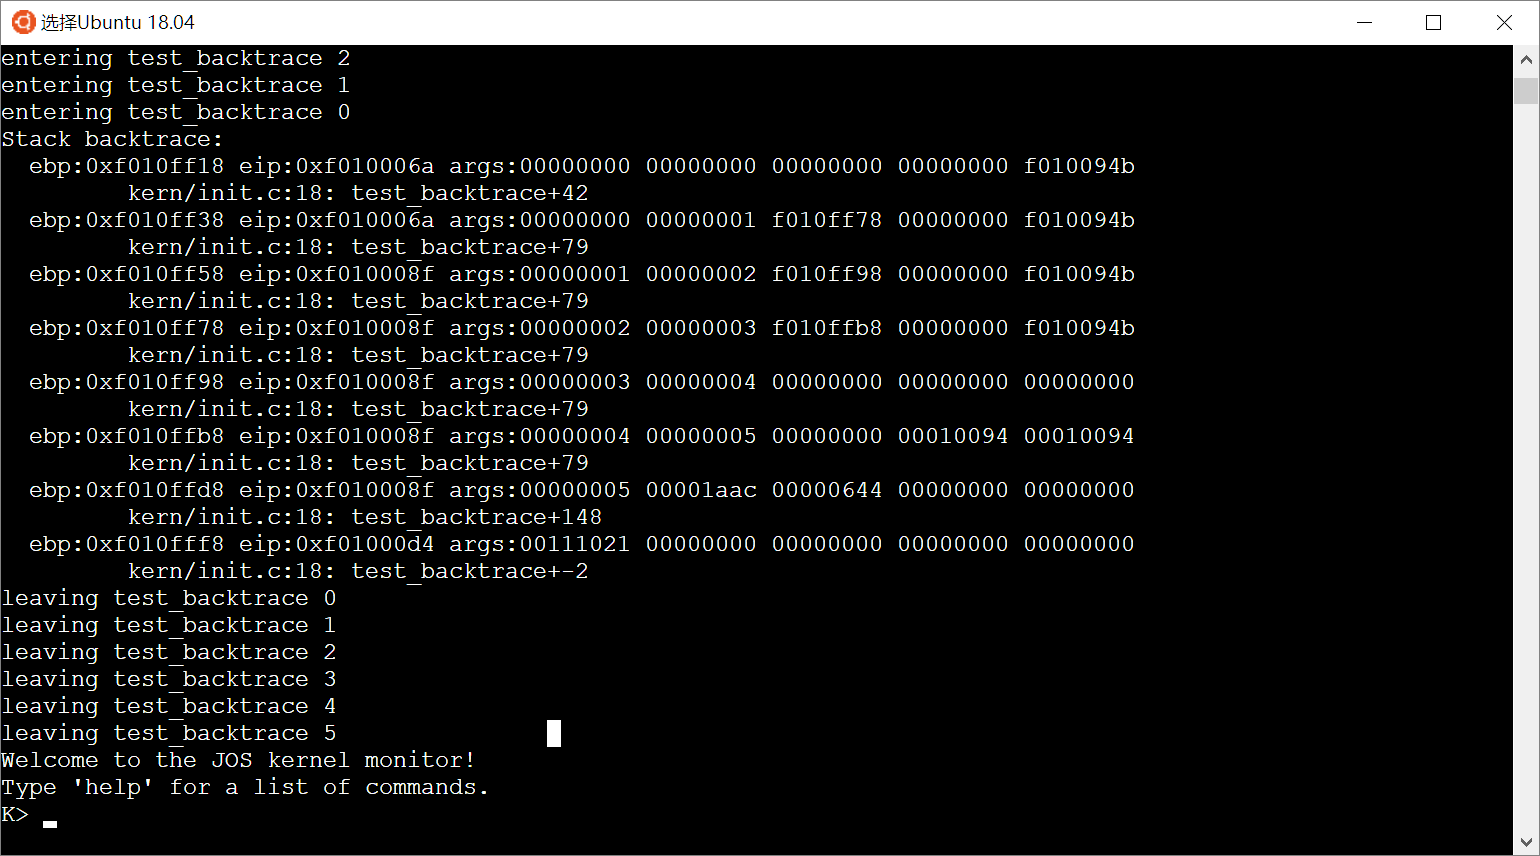
\includegraphics[width = .85\linewidth]{img/ch.png}
    \caption{挑战作业实验结果}
    \label{fig::figurech}
\end{figure}


% \bibliography{lab1_1}


\end{document}